\mysection{System Sensitivity Analysis}\label{sensitivityAnalyis}

Next up we are going to find out how sensitive or robust the system is to a change in event input sizes.
Furthermore, we want to know where possible bottlenecks are and how to choose optimal processor or bus dimensions.

\mysubsection{How robust is the system?}

A robust system is not sensitive towards changes in the event stream rates:
An increase of the input data rate of any event stream by a few percents does not cause significant changes in the systems end-to-end delays~\cite{wan:06}.
Specifically the new end-to-end delays to not exceed the specified maximum delay times of the system applications.
In order to increase the system's robustness we need to look for and eliminate bottlenecks.

\mysubsection{Where is the bottleneck?}

The resource, that the system is most sensitive to, when changing its capacity, is a potential bottleneck resource.
If we now slightly higher the capacity of a bottleneck resource,
without chancing the capacities of any other resources, the end-to-end delay of at least one event stream immediately decreases, and therefore the system quality increases~\cite{wan:06}.

\mysubsection{Using the Results of MPA to Make Design Decisions: Improving Architectures}

When designing a new embedded real-time system, we want to find out what architecture works best for the specific use case.
Therefore, we want to try out numerous possible system models and compare them in therms of their performances and robustness.
\autoref{performanceAnalysis} and \autoref{sensitivityAnalyis} give us a great opportunities to do so, using the system performance model.
We can now quickly propose, analyze and compare various systems.
These systems may be extremely different, for example when trying out opposed architectures, or just slightly different, for example when decreasing a CPU's
performance by just a few percent to see if we can make the system cheaper, without risking any disadvantages.
Additionally, we can try out different scheduling strategies or change
the communication structure between the resources, to develop new, and thus maybe improved, system models~\cite{wan:06}.

In the end it is the goal to find a system that, fulfills the timing requirements of all applications
and is robust enough in respect to changes,
while being as cheap as possible and therefore as small-dimensioned as possible.

\mysubsection{Sensitivity Analysis of the Sample System}

After we chose architecture A to be sufficient to the timing requirements in \autoref{performanceAnalysis}, we now want to investigate on the
architecture's robustness and further improve it.
With \autoref{fig:robust-A} and \autoref{fig:robust-B} we realize that the architecture is actually quite robust to increasing event stream rates,
yet it is unable to handle more than 20 brightness events per second or more than 4 message events per second.

Increasing the capacities of CPU1 (\autoref{fig:bottleneck-B1}), the bus (\autoref{fig:bottleneck-B2}) or CPU2 (\autoref{fig:bottleneck-B3}),
all immediately lead to improved delays, at least when it comes to message events.
As the delays decrease the fastest, when increasing the resource capacity of CPU3, we choose this resource to be worthy of further improvements.

\begin{figure}
    \centering
    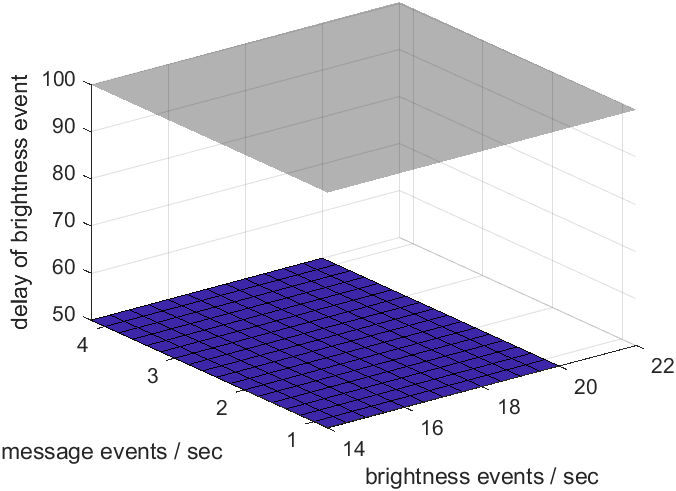
\includegraphics[width=0.8\columnwidth]{graphics/robustA.png}
    \caption{Impacts associated to increasing the rate of \(\alpha_{Brightness}\)}\label{fig:robust-A}
\end{figure}

\begin{figure}
    \centering
    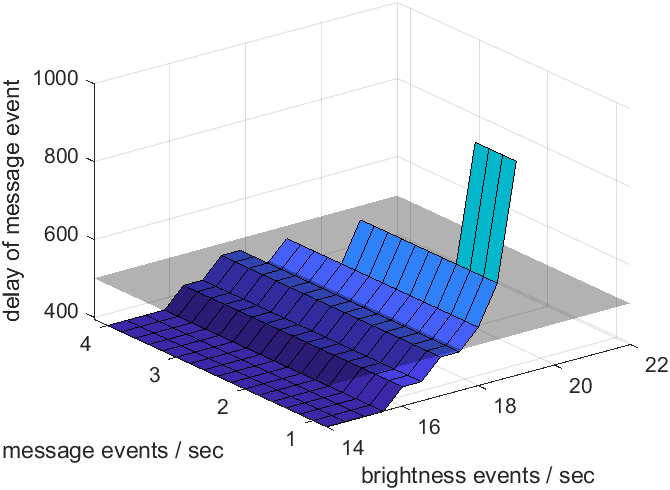
\includegraphics[width=0.8\columnwidth]{graphics/robustB.png}
    \caption{Impacts associated to increasing the rate of \(\alpha_{Message}\)}\label{fig:robust-B}
\end{figure}

\begin{figure}
    \centering
    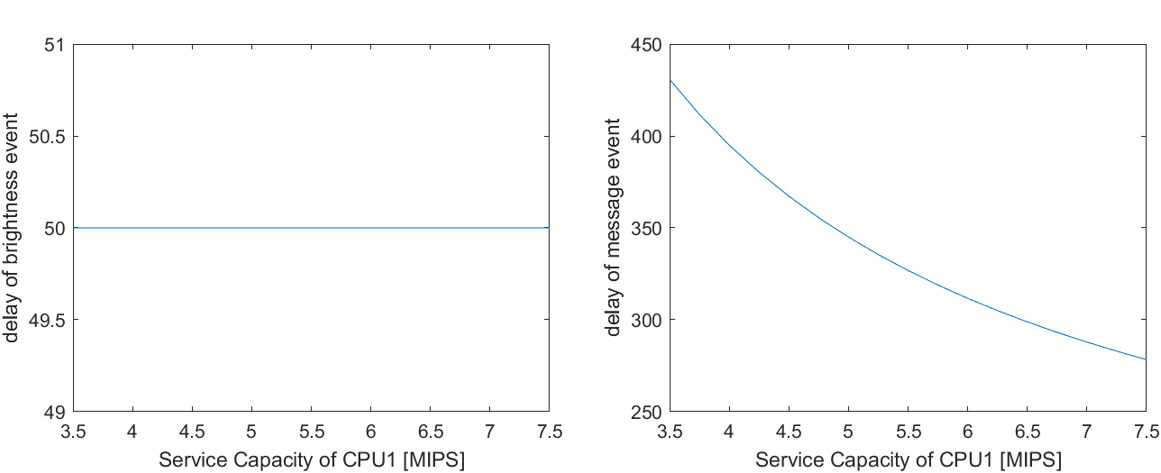
\includegraphics[width=\columnwidth]{graphics/bottleneckB1.png}
    \caption{Impacts associated to increasing the service capacity of CPU1}\label{fig:bottleneck-B1}
\end{figure}

\begin{figure}
    \centering
    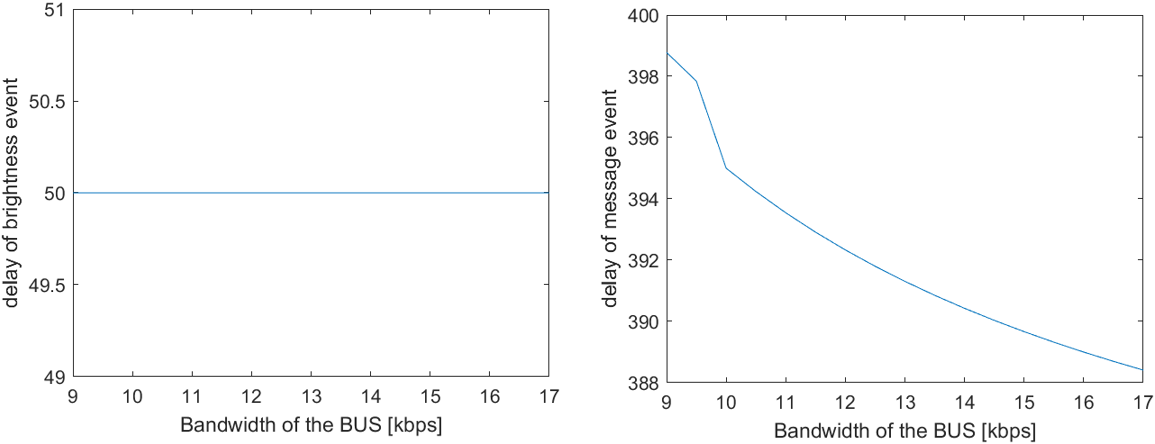
\includegraphics[width=\columnwidth]{graphics/bottleneckB2.png}
    \caption{Impacts associated to increasing the bandwidth of the BUS}\label{fig:bottleneck-B2}
\end{figure}

\begin{figure}
    \centering
    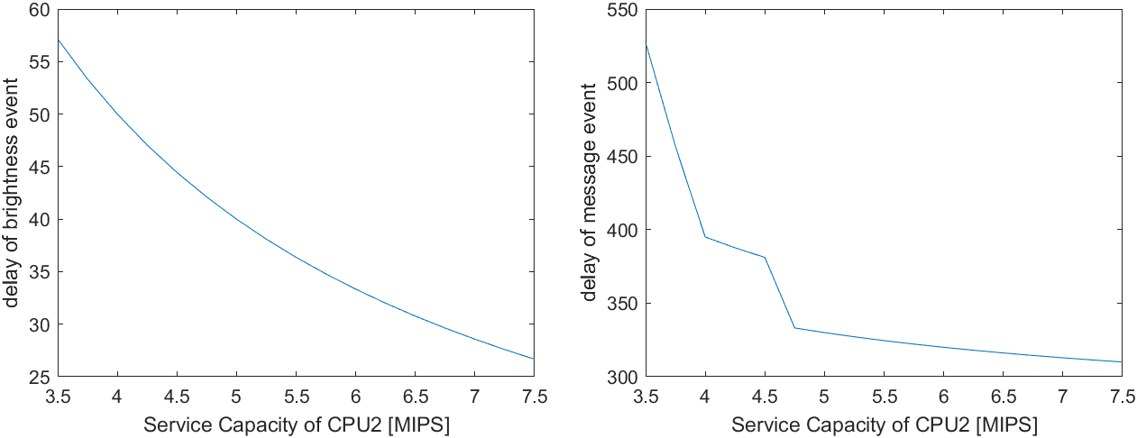
\includegraphics[width=\columnwidth]{graphics/bottleneckB3.png}
    \caption{Impacts associated to increasing the service capacity of CPU2}\label{fig:bottleneck-B3}
\end{figure}